To understand the structure and evolution of the universe, astrophysicists must measure not just light, but mass. Stars, galaxies, and gas clouds emit radiation that reveals their presence, but the dynamics of the cosmos are governed by gravity — by how much mass exists and how it is distributed. Knowing where matter is, and how much of it there is, is necessary for explaining motion, structure formation, and stability across cosmic scales. The question is: how can one measure mass across millions of light-years, when most of it emits no light at all?

The primary method is to observe motion. In Newtonian mechanics, any orbiting body experiences a centripetal acceleration that is directly related to the mass it orbits. This relationship allows astronomers to determine how much mass lies within a given radius, provided they can measure orbital speeds and distances. By measuring the velocities of stars at different radii from the center of a galaxy, astrophysicists can infer how mass is distributed throughout the galaxy — not just in its luminous regions.

Spectroscopy plays a central role in this process. When light from a star or gas cloud is dispersed into its component wavelengths, the resulting spectrum reveals its motion via Doppler shifts. A redshift indicates motion away from the observer; a blueshift indicates motion toward. These shifts allow for measurements of velocity along the line of sight. Rotational velocities within galaxies, random velocities in galaxy clusters, and internal turbulence in gas clouds can all be extracted from spectral line profiles.

Radio astronomy extends these measurements beyond visible light. Neutral hydrogen, the most abundant element in the universe, emits radiation at a wavelength of 21 centimeters. This emission can be traced even in the outskirts of galaxies, where stars are sparse or absent. Observing the motion of this gas provides crucial data on gravitational effects well outside the luminous core. These measurements have been central to mapping galactic dynamics.

In systems without a simple rotation pattern — such as elliptical galaxies or clusters — mass is inferred statistically. The velocities of constituent bodies follow distributions governed by the overall gravitational potential. In these cases, the virial theorem (as is explored also in the chapter on osmosis) connects the average kinetic energy of the system to the total mass required to confine it. This technique is especially important in estimating the masses of galaxy clusters, where galaxies orbit in all directions and the system behaves like a gravitationally bound swarm.

A complementary approach bypasses dynamics altogether: gravitational lensing. According to general relativity, mass curves spacetime, bending the path of light from background sources. When a massive object — such as a galaxy or cluster — lies along the line of sight to a more distant source, the background light is distorted. By analyzing the shape and degree of this distortion, one can map the total mass distribution of the intervening object. This method is purely gravitational: it measures mass regardless of whether it emits, absorbs, or reflects light.

When mass in a galaxy is concentrated toward the center, orbital velocities should decrease with distance, just as planets in the Solar System orbit more slowly the farther they are from the Sun. This prediction follows directly from Newtonian dynamics: outside a spherically symmetric mass distribution, the gravitational force behaves as if all mass were concentrated at the center. Applied to galaxies, this implies that rotational velocity should drop off with radius beyond the visible stellar disk. Observations do not match this expectation. In spiral galaxies, stars orbit the center at nearly constant speed over vast radial distances. These flat rotation curves indicate that the enclosed mass does not level off where the stars end, but continues to increase. The luminous matter — stars, gas, and dust — cannot account for this excess gravity.

The persistence of high orbital speeds well beyond the visible edge of galaxies is confirmed by radio observations of neutral hydrogen. Radio telescopes can map the velocity of this gas across the outskirts of galaxies. These measurements show that rotational velocities remain flat or even rise at large radii, where the density of luminous matter has dropped to negligible levels. The simplest explanation is that galaxies are embedded in extended halos of non-luminous mass, whose gravitational influence dominates in the outer regions.

On larger scales, galaxy clusters present an analogous discrepancy. These systems contain hundreds or thousands of galaxies bound together by gravity, along with large amounts of hot gas that emits strongly in X-rays. The temperature and distribution of this gas reflect the depth of the gravitational potential well. If only the visible galaxies and gas contributed to the cluster’s gravity, the hot gas would escape over cosmological timescales. That it remains bound implies a much larger total mass than what is seen. The internal motions of galaxies within clusters, measured by redshift dispersion, independently confirm this excess mass. Gravitational lensing applies also to these massive clusters, and in both context (individual galaxies and clusters), the lensing signal supports the presence of a dominant, unseen mass component.

A unique astrophysical event — \textbf{the Bullet Cluster} — provides direct evidence for a non-luminous mass component that behaves differently from ordinary matter. This system consists of two galaxy clusters in the process of collision. As they pass through one another, the hot gas from each cluster interacts and slows down due to ram pressure (the force of the bulk motion. Compare to temperature, the other kinetic component, in the chapter about negative temperature), becoming spatially displaced from the galaxies themselves. X-ray observations reveal this gas concentrated between the clusters. However, gravitational lensing maps of the same region show that most of the mass is still centered on the galaxies, not the gas. This separation implies that the dominant mass component did not experience significant drag during the collision. It must interact gravitationally, but not electromagnetically — suggesting it is both massive and effectively collisionless.

The early universe provides a separate window into the distribution of mass through the spectral composition of the cosmic microwave background. This radiation carries a record of acoustic oscillations in the primordial plasma — pressure waves driven by the interplay between gravity and radiation. The pattern of these oscillations, visible as peaks in the CMB power spectrum, depends sensitively on the matter content of the universe. Ordinary (baryonic) matter couples to photons and thus participates in pressure waves, while non-baryonic matter does not. Matching the observed amplitude and spacing of the peaks requires a dominant component of matter that does not interact with radiation, but contributes to gravitational attraction. Precision measurements by the WMAP and Planck satellites confirm that ordinary matter accounts for only a small fraction of the total.

Numerical simulations of structure formation reinforce this conclusion. Starting from the nearly uniform density field observed in the CMB, simulations track the growth under gravity. The timing and scale of galaxy and cluster formation are highly sensitive to the amount and type of matter present. If only ordinary matter were included, structure would form too slowly to match what is observed in deep-field surveys. The emergence of galaxies, clusters, and the cosmic web within a few billion years requires a gravitational source that was present from the earliest epochs, unaffected by radiation pressure, and capable of seeding the collapse of matter on small scales. The observed universe forms on schedule only when this additional component is included.

Thus, the evidence for dark matter does not rest on a single anomalous measurement, but on the convergence of diverse and independent observational domains. Galaxy rotation curves, cluster dynamics, X-ray temperature profiles, gravitational lensing, and the cosmic microwave background all indicate that visible matter accounts for only a small fraction of the gravitational forces at work. The required additional mass must act through gravity, but not through electromagnetism; it must clump on galactic scales, but remain diffuse enough not to obstruct light; it must have existed before the era of recombination, but not interfered with photon-matter coupling. The simplest explanation consistent with all constraints is the existence of a non-luminous, cold, and effectively collisionless form of matter — distinct from atoms, but essential for the cosmic configuration.

Attempts to resolve these discrepancies by modifying the laws of gravity instead of introducing a new kind of matter have achieved only partial success. Modified Newtonian dynamics (MOND) can account for some features of galactic rotation curves, but struggle with systems lacking clear symmetry or equilibrium. The Bullet Cluster, in particular, presents a direct conflict: the separation of gravitational and luminous mass cannot be explained by alterations to the gravitational field alone. Gravitational lensing imposes geometric constraints that any alternative theory must satisfy, and these constraints are difficult to reconcile with models that dispense entirely with unseen mass. The full range of phenomena — from early-universe fluctuations to present-day structure — aligns with the presence of a real, additional matter component, much better than by a reformulation of force laws.

\newpage

\vspace{2em}

\begin{center}
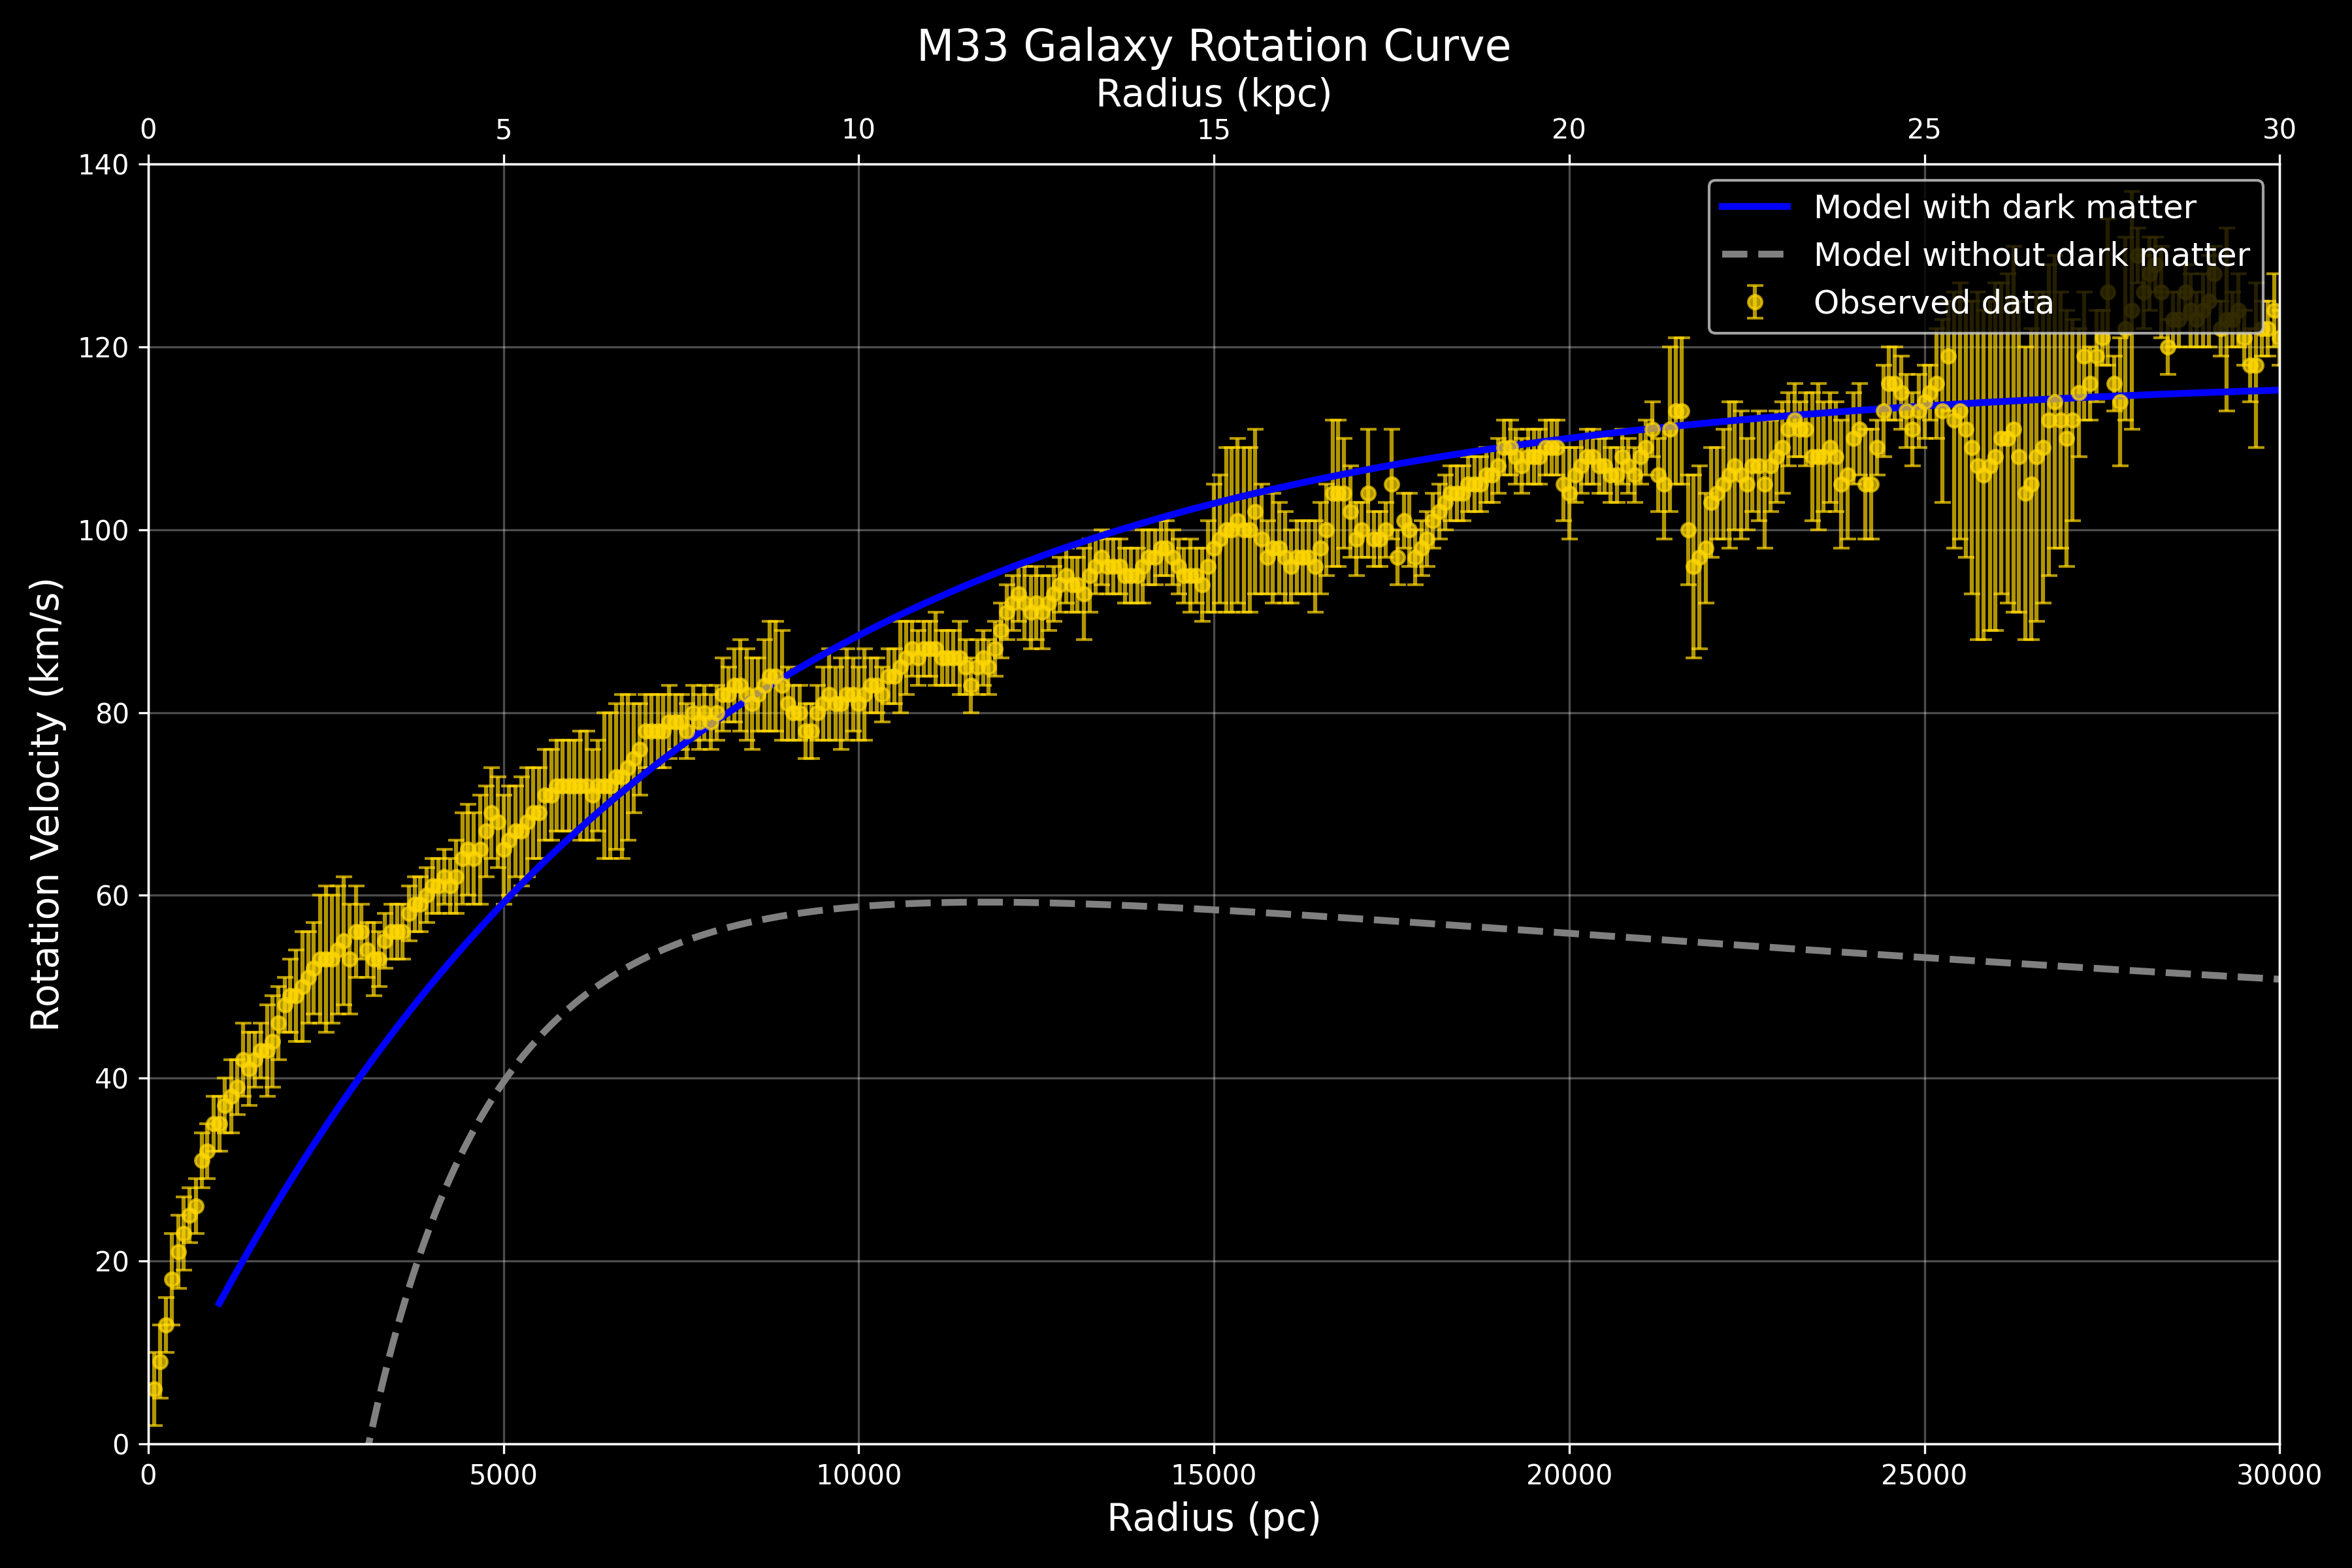
\includegraphics[width=0.75\textwidth]{37_DarkMatterEvidence/m33_rotation_curve.png}    \\
\textbf{M33 Galaxy Rotation Curve.} The rotation curve of the M33 galaxy (Triangulum Galaxy) demonstrates the need for dark matter in galaxies. Yellow points represent observed H$\alpha$ spectroscopic data collected at the Observatoire du Mont Megantic, showing rotation velocities with error bars at different galactocentric radii. The solid blue line shows a model that includes dark matter contribution, following the function $v = M \cdot (1 - e^{-r/R})$, which maintains high velocities at large radii. The gray dashed line represents a toy model based only on visible baryonic matter which cannot account for the observed rotation velocities in the outer regions of the galaxy. This discrepancy provides compelling evidence for the presence of a dark matter halo extending far beyond the visible disk of M33.

\vspace{0.5em}
\small{Figure generated by me using data points from Kam et al. (2015), "The H$\alpha$ rotation curve of M33" (MNRAS, 449, 4048). The fitted curved are not from the literature and for illustrative purposes only.}
\end{center}
